\chapter{No Linealidad Material}\label{cap3MNA}
%
En este capítulo se introducen herramientas básicas para el análisis de estructuras considerando no linealidad material, es decir relaciones no lineales entre tensiones y deformaciones. %
%
Se comienza presentando las ecuaciones para el análisis de estructuras de barras con relación tensión-deformación elástica no lineal, para luego pasar a introducir elementos básicos de la teoría de plasticidad.

\section{Elasticidad no lineal} \label{sec:hiper}

En esta sección se describen de forma sintética los conceptos básicos del análisis elástico considerando un comportamiento constitutivo no lineal, en particular el dado para sólidos hiperelásticos. %
%
A partir de esto se presentan las ecuaciones para estructuras de barras articuladas con comportamiento elástico no lineal. %
%
Se omitirán numerosas consideraciones teóricas importantes para el análisis de sólidos, las cuales se pueden encontrar en textos como \citep{Holzapfel2000a,Gurtin1981}.
% --------------------------------------

\subsection{Hiperelasticidad en sólidos} %
%

\subsubsection{Aspectos básicos}

Se considera un sólido que ocupa, en la configuración de referencia, la región $\Omega_0 \subset \bbR^3$, cuyo contorno es unión disjunta de $\Gamma_\bff$ y $\Gamma_\bfu$ ($\partial \Omega_0 = \Gamma_{\bfu} \cup \Gamma_{\bff}$ y $\Gamma_{\bfu} \cap \Gamma_{\bff} = \emptyset$)
, donde existe desplazamiento impuesto en $\Gamma_\bfu$ y tensiones externas $\bft_{\text{ext}}$ aplicadas en $\Gamma_\bff$. %
%
El Problema de Elasticidad no Lineal para sólidos consiste en encontrar la configuración deformada del cuerpo $\Omega_t$ de forma tal de minimizar la energía potencial total. %

Cada partícula $P$ del sólido ocupa una posición $\bfx_0$ en la configuración de referencia. %
%
En el instante de tiempo $t$ (o más formalmente para el factor de carga correspondiente a $t$) cada partícula $P$ pasa a ocupar una posición dada por el vector $\bfx_t$ el cual pertenece al conjunto de la configuración deformada $\Omega_t$. %
%
Se establece que existe una función $\chi:\Omega_0\times \bbR^+ \rightarrow \Omega_t$ que relaciona las posiciones en la configuración de referencia con las posiciones deformadas de la forma:
%
\begin{equation}
\bfx_t = \chi(\bfx_0,t).
\end{equation}
%
La función $\chi$ debe cumplir un conjunto de hipótesis relevantes que no serán consideradas en este documento, entre las que se menciona la biyectividad. %


%
Se define el campo vectorial de desplazamientos para el instante $t$, denotado como $\bfu_t:\Omega_0\rightarrow \bbR^3$, a través de la siguiente expresión:
%
\begin{equation}
\bfu_t(\bfx_0) = \bfx_t - \bfx_0.
\end{equation}
%
La dependencia de $t$ está dada de forma implícita a través del subíndice. %
%
El útil calcular el gradiente de dicho campo denotado por $\bfD$ cuya expresión se obtiene derivando ambos miembros respecto a $\bfx_0$:  
%
\begin{equation}\label{eqn:eqF}
\bfD (\bfx_0) = \bfF(\bfx_0) - \bfI,
\end{equation}
%
donde $\bfF$ es un tensor llamado gradiente de deformación dado por:
%
\begin{equation}\nonumber
\bfF(\bfx_0) = \dfrac{\partial \bfx_t}{\partial \bfx_0}(\bfx_0).
\end{equation}
%
%
Dado que se considera la deformada en un único instante, se omitió el tiempo $t$ así como también se podrá omitir la evaluación en el punto $\bfx$ de ahora en adelante. %
% -----------------------------------------------



%\subparagraph{Estado de Deformaciones .}
Sean dos puntos $\bfx_0$ y $\hat{\bfx}_0$ cercanos de la configuración de referencia y sus correspondientes puntos deformados $\bfx_t$ y $\hat{\bfx}_t$. %
%
Utilizando la definición de $\chi$ y realizando un desarrollo de primer orden respecto a $\bfx_0$ se obtiene la relación:
% 
\begin{equation} \label{eqn:relchi}
\hat{\bfx}_t - \bfx_t = \chi(\hat{\bfx}_0,t) - \chi(\bfx_0,t) \simeq \bfF(\bfx_0)(\hat{\bfx}_0-\bfx_0),
\end{equation}
%
donde se consideró que la distancia entre los puntos $\bfx_0$ y $\hat{\bfx}_0$ es pequeña. %
%
Esta identidad permite tener una relación entre los segmentos en las configuraciones de referencia y deformada.
%
La magnitud escalar $J(\bfx_0) = |\bfF(\bfx_0)|$ representa la razón de variación volumétrica local en un entorno de la partícula que ocupa la posición $\bfx_0$ en la configuración de referencia. %
%
La función de deformación $\chi$ debe cumplir ciertas hipótesis de continuidad, como por ejemplo verificar que la razón de variación volumétrica sea positiva durante todo el movimiento. %Esto está asociado a la no interpenetración del cuerpo. %
%


El estado local de deformaciones en un entorno de $\bfx_0$ está definido por lo tanto por el tensor $\bfF$, sin embargo existen diferentes definiciones de tensores que permiten representar el estado de deformaciones local. %
%
Una herramienta útil es el tensor de deformaciones de Green $\bfE$ el cual será definido de forma simplificada como una extensión de la definición considerada para elementos de barra. %
%

Se consideran los segmentos $d\bfx_0$ y $d\bfx_t$ dados por:
\begin{equation}\label{eqn:relF}
\hat{\bfx}_0 - \bfx_0 = d\bfx_0 \qquad \text{y} \qquad \hat{\bfx}_t -\bfx_t = d\bfx_t.
\end{equation}
%
Se desea aplicar la definición de la deformación de Green para calcular la expresión de la deformación unitaria del segmento $d\bfx_0$, esto es:
%
\begin{equation}
\varep_{d\bfx_0} = \frac{1}{2} \frac{d\bfx_t^{\text{T}} d\bfx_t - d\bfx_0^{\text{T}} d\bfx_0} {d\bfx_0^{\text{T}} d\bfx_0}.
\end{equation}
%
Por otra parte los segmentos $d\bfx_t$ y $d\bfx_0$ están relacionados a través de la Ecuación~\eqref{eqn:relchi} y las expresiones la Ecuación~\eqref{eqn:eqF}, por lo que se obtiene:
%
\begin{equation}
\varep_{d\bfx_0} = \frac{1}{2} d\bfx_0^{\text{T}} \left( \bfF^{\text{T}} \bfF - \bfI\right) d\bfx_0.
\end{equation}
%
Por lo que definiendo el tensor de deformaciones de Green como:
%
\begin{equation}
\bfE = \frac{1}{2} \left( \bfF^{\text{T}} \bfF - \bfI\right),
\end{equation}
%
se obtiene la siguiente expresión simplificada de la deformación unitaria:
\begin{equation}
\varep_{d\bfx_0} = d\bfx_0^{\text{T}} \bfE d\bfx_0.
\end{equation}

Se puede ver que la matriz asociada de $\bfE$ es simétrica por lo que tendrá valores propios reales. %
%
Estos valores propios representan las deformaciones unitarias de Green correspondientes a los segmentos dados por las direcciones principales. %
% ------------------------------

Sustituyendo la expresión de $\bfF$ en función del gradiente de desplazamiento dada por la Ecuación~\eqref{eqn:eqF} se obtiene
%
\begin{equation}
\bfE = \frac{1}{2} \left( \bfD + \bfD^{\text{T}} + \bfD^{\text{T}} \bfD \right).
\end{equation}
%
Se puede ver que tal como ocurre en el caso de barras, al considerar pequeñas deformaciones se obtienen equivalencias entre distintas medidas de deformación. %
%
En el caso de la medida de Green, al considerar las componentes de primer orden se obtiene:
\begin{equation}
\bfE \simeq \frac{1}{2} \left(  \bfD + \bfD^{\text{T}} \right) = \bfvarep, 
\end{equation}
%
donde $\bfvarep$ es el tensor de deformaciones infinitesimales asociado a la medida de deformación presentada en el capítulo anterior como deformación ingenieril.
% --------------------------------------------



\subsubsection{Material Hiperelástico}

Un material es elástico si y solo sí las tensiones internas producidas en el sólido dependen únicamente de la deformación actual. %
%
En el caso de un material hiperelástico, existe una función escalar, llamada densidad de energía de deformación interna, $\Psi(\bfE):\text{Sym}\rightarrow \bbR $, la cual determina el comportamiento constitutivo a través de la relación 
%
\begin{equation}
\bfS = \frac{\partial \Psi}{ \partial \bfE } (\bfE),
\end{equation}
donde $\bfS$ es el tensor de tensiones de Cosserat (o segundo tensor de Piola). %
%
Este campo tensorial está definido en puntos de la configuración de referencia y representa una de las posibles medidas de tensión a o utilizar. %
Por otra parte, el tensor de tensiones de Cauchy $\bfsig$ está definido en la configuración deformada y está relacionado con $\bfS$ a través de la expresión:
%
\begin{equation}
\bfS = J \bfF^{-1} \bfsig \bfF^{-T}.
\end{equation}
%

%
Esta función de densidad de energía de deformación permite calcular el total de energía potencial elástica $U$ acumulada por el cuerpo al ser sometido a un desplazamiento $\bfu$, a través de la expresión:
%
\begin{equation}
U(\bfu) =  \frac{1}{2} \int_{\Omega} \Psi (\bfE( \bfu ) ) \, \dif V.
\end{equation}
%
% ----------------------------------------------------


%\subparagraph{Mínima energía .} %
Tal como fue presentado en el capítulo anterior, el equilibrio está asociado a la configuración donde la energía potencial total $V$ es mínima, por lo que el problema de hallar la configuración de equilibrio consiste en un problema de optimización no lineal: %
%
%
\begin{equation}\label{eqn:prelim_minetot}
\min_{\bfu \in \mcU} \quad  U(\bfu) - \int_{\Gamma_{\bff}} \bfu^{\text{T}} \bft_{\text{ext}} \dif A,
\end{equation}
%
donde $\mcU$ es el conjunto de desplazamientos cinemáticamente admisibles, es decir compatibles con los vínculos externos. %

Al igual que en el caso de barras, las condiciones de optimalidad del problema llevan al principio de trabajos virtuales, donde las fuerzas internas están dadas por integrales en el volumen de la densidad de trabajo virtual de las tensiones internas, dadas por el producto escalar del tensor de tensiones y el tensor de deformaciones virtuales $\bfS:\delta\bfE$. %
%
Al igual que en el caso de elementos de barras existen diversos métodos numéricos que permiten resolver el problema, entre los que se encuentran algoritmos de optimización no lineal.
% ------------------------------



% --------------------------------------
\subsubsection{Funciones $\Psi$ para materiales compresibles}
%
%\subparagraph{Intro .}
Dado que el comportamiento del material es determinado por la función $\Psi$ se presentan un par de ejemplos de funciones propuestas para modelar el comportamiento constitutivo de sólidos isótropos. %
% ----------------------------

%
\paragraph{Saint-Venant Kirchoff}
El modelo de Saint-Venant-Kirchhoff establece una relación lineal entre el tensor de Cosserat y el tensor de deformaciones de Green. La expresión matemática de $\Psi$ en este caso es:
%
\begin{equation}
\Psi (\bfE) = \frac{\lambda}{2} \tra(\bfE)^2 + \mu \tra(\bfE^2),
\end{equation}
%
donde $\lambda$ y $\mu$ son dos parámetros reales del modelo que caracterizan el comportamiento del material. %
%
Esta función establece entonces una expresión para las tensiones en todo punto a partir de la deformación, dada por:
%
\begin{equation}\label{eqn:eqconssvk}
\bfS = \lambda \tra(\bfE) \bfI + 2 \mu \bfE .
\end{equation}
%
Este modelo corresponde a la ley lineal considerada en el capítulo anterior para barras con medida de deformación de Green. %
%
En el caso de pequeñas deformaciones este modelo lleva a la conocida ley constitutiva de Hooke.
% ---------------------------


\paragraph{Curnier}
%
El modelo de Saint-Venant-Kirchoff permite representar el comportamiento a tracción para grandes deformaciones aunque no es capaz de proveer buenos resultados en compresión ya que, como fue visto, se produce una pérdida de rigidez. %
%
En \citep{Curnier1994} (ver Sección 6.6.2) se describe un modelo modificado capaz de representar estados de compresión en grandes deformaciones. %
%
La expresión de la densidad de energía de deformación es:
%
\begin{equation}
\Psi (\bfE) = \lambda (J - \log(J)-1 ) + \mu \tra(\bfE^2),
\end{equation}
%
siendo el tensor de Cosserat en este caso dado por:
%
\begin{equation}
  \bfS = \lambda ( J-1 ) \bfF^{-1} \bfF^{-T}  + 2 \mu \bfE.
\end{equation}
%


\subsubsection{Funciones $\Psi$ para materiales incompresibles}
%
Existen materiales con un comportamiento constitutivo tal que se requieren elevadas cantidades de energía para poder realizar deformaciones asociadas a variaciones de volumen, es decir que las deformaciones que efectivamente desarrolla el sólido cumplen $J=1$ en todo punto. %
%
Estos materiales son llamados incompresibles y no serán considerados en este documento ya que su uso no es considerablemente frecuente en soluciones estructurales. %

Materiales como polímeros suelen ser analizados con este tipo de modelos por lo que el comportamiento de algunos elementos estructurales puede ser estudiado con este tipo de funciones $\Psi$. %
%
Existe una gran variedad de funciones de energía utilizadas en diversas aplicaciones, como por ejemplo: el modelo \textit{Neo-Hookean} uno de los más simples (ver \citep{Holzapfel2000a}), el modelo presentado por \cite{Delfino1997} apropiado para el modelado de ciertos comportamientos observados experimentalmente en arterias carótidas o el modelo de \cite{Veronda1970} el cual fue aplicado para el desarrollo de una técnica de diagnóstico de tumores malignos en mamas \citep{Goenezen2012}.


\subsubsection{Pequeñas deformaciones}

En el caso de pequeñas deformaciones se tiene que el tensor $\bfE$ es aproximadamente igual a $\bfvarep$ y que el tensor de tensiones $\bfS$ es aproximadamente igual al tensor de tensiones de Cauchy $\bfsig$ en coordenadas locales (sistema co-rotacional) por lo que la definición de material hiperelástico puede ser considerada ahora como:
%
\begin{equation}
  \bfsig = \frac{\partial \psi}{\partial \bfvarep} (\bfvarep).
\end{equation}
%
No serán abordadas en este documento las condiciones que debe cumplir la función $\psi$, sin embargo se considerará que deberán ser funciones que garanticen al menos continuidad de la función $\bfsig(\bfvarep)$. %
%
Esta función determina la nolinealidad material para comportamiento elástico en pequeñas deformaciones.


En el caso del material de Saint-Venant-Kirchhoff para pequeñas deformaciones se obtiene una expresión de $\psi$ dada por:
%
\begin{equation}
\psi(\bfvarep) = \frac{\lambda}{2} \left( \text{Tr}(\bfvarep)\right)^2 +  \mu \left(\text{Tr}(\bfvarep^2)\right)
\end{equation}
%
y la relación del tensor de tensiones está dada por:
%
\begin{equation}
\bfsig = \frac{\partial \psi}{\partial \bfvarep} (\bfvarep) = \lambda \text{Tr}(\bfvarep) +  2 \mu \bfvarep,
\end{equation}
lo que coincide con la ecuación constitutiva del material elástico-lineal. %
%


\subsection{Hiperelasticidad en barras}

En el caso de barras con comportamiento hiperelástico el estado tensional corresponde a un estado uniaxial de tensiones. %
%
En \citep{Castrillo2014} se presenta la resolución de diversos ejemplos de reticulados tridimensionales con comportamiento hiperelástico para el material de Saint-Venant-Kichhoff deduciendo las soluciones a partir de las ecuaciones válidas para sólidos. %
%

Si un eje del sistema de coordenadas coincide con el eje de la barra entonces la componente asociada a dicha dirección será la única entrada no nula dada por
%
\begin{equation}
\sigma_x = \frac{\partial \psi}{\varepsilon_x}(\varepsilon_x) = \sigma (\varepsilon_x),
\end{equation}
%
por simplicidad se considerará que la tensión está dada por la función $\sigma(\varepsilon)$. %



% -------------------------
En el capítulo anterior se presentaron las ecuaciones del PTV, cuya aplicación lleva al sistema de ecuaciones no lineales:
%
\begin{equation}
  \bff_{\text{int}}(\bfu) - \bff_{\text{ext}} = \bszer.
\end{equation}
% ------------------
%
Para el desarrollo de los métodos numéricos la resolución de estas ecuaciones se asumió una relación constitutiva lineal. %
%
Si se continúa el desarrollo desde la Ecuación~\eqref{eqn:fueinterna} y considerando ahora una relación general no lineal entre tensión y deformación, se tiene:
%
\begin{equation}
\frac{\partial \bff^e_{\text{int}} } {\partial \bfu^e} (\bfu^{(k)}) 
= A_0^e \ell_0^e \left( \frac{\partial \bfb^e}{\partial \bfu^e} (\bfu^{(k)}) \right)^{\text{T}} \sigma^e(\varep((\bfu^{(k)})))
+ A_0^e \ell_0^e  (\bfb^e(\bfu^{(k)}))^{\text{T}} \frac{ \partial \sigma^e}{\partial \bfu^e}( \varep( \bfu^{(k)}) ).
\end{equation}

Usando la función del comportamiento no lineal y la regla de la cadena se tiene:
\begin{equation}
\frac{ \partial \sigma}{\partial \bfu}(\bfu) = E^{\text{tan}}(\varep(\bfu)) \frac{ \partial \varep}{\partial \bfu}(\bfu)
\end{equation}
donde $E^{\text{tan}}$ es el llamado módulo tangente, dado por:
\begin{equation}
E^{\text{tan}}(\varep) = \frac{ \partial \sigma}{\partial \varep} (\varepsilon).
\end{equation}

Sustituyendo en la ecuación de la derivada de las fuerzas internas se tiene:
\begin{equation}
\frac{\partial \bff_{\text{int}}^e } {\partial \bfu^e} (\bfu^{(k)})
= \frac{\sigma ( \varep( \bfu^{(k)}) ) A_0 }{\ell_0} \bfG^e
+  (\bfb^e(\bfu^{(k)}))^{\text{T}} \,  E^{\text{tan}} (\varepsilon(\bfu^{(k)})) A_0^e \ell_0^e \, \bfb^e(\bfu^{(k)}).
\end{equation}

El proceso de ensamblado de la matriz tangente y resolución del método Newton-Raphson es similar al realizado para análisis con nolinealidad geométrica, teniendo en cuenta que el vector de fuerzas internas debe ser calculado con la tensión dada por la relación no lineal.


La herramienta ONSAS permite que el usuario introduzca cualquier modelo hiperelástico para el comportamiento de las barras a través de la función \textit{hyperElasModels}.


\subsection{Análisis de reticulados bi-modulares}



%\subsection{Condiciones de optimalidad KKT}
%
%
%\begin{equation}
%\left\{
%\begin{array}{l}
%\min_{x} \qquad  f(x)\\
%\text{s.a.}\\
%\quad g(x)\leq 0\\
%\quad h(x) = 0
%\end{array}
%\right.
%\end{equation}
%
%
%
%\begin{equation}
%\left\{
%\begin{array}{l}
%\nabla f(x) + \lambda \nabla g(x) + \mu \nabla h(x) = 0\\
%g(x)\leq 0\\
%h(x) = 0\\
%\lambda \geq 0\\
%\lambda g(x) = 0
%\end{array}
%\right.
%\end{equation}


Existe un grupo importante de materiales llamados bi-modulares (en ingles \textit{bi-modulus materials}), los cuales se caracterizan por tener diferente comportamiento constitutivo a tracción y a compresión. %
%
Entre algunos ejemplos se encuentran la madera y el hormigón, cuyo análisis simplificado es generalmente realizado sin tomar en cuenta esta no linealidad. %
%

Por otra parte en elementos estructurales como cables o tensores se puede considerar que el elemento no soporta esfuerzos de compresión, lo que puede modelarse como un comportamiento constitutivo no lineal para desplazamientos pequeños.
% 

\subsubsection{Abordaje mediante PTV y métodos iterativos}

El abordaje asociado al PTV y los correspondientes métodos iterativos pueden ser aplicados considerando la función $\sigma$ y su derivada en las ecuaciones de PTV y los correspondientes métodos numéricos. Estas expresiones son: %
%
\begin{equation}
\sigma (\varepsilon) = 
\left\{
\begin{array}{lr}
E_T \varepsilon & \text{si } \varep \geq 0 \\
E_C \varepsilon & \text{si }\varep <0
\end{array}
\right.
\qquad
\frac{\partial \sigma}{\partial \varep} (\varepsilon) = 
\left\{
\begin{array}{lr}
E_T & \text{si }\varep \geq 0 \\
E_C & \text{si }\varep < 0
\end{array}
\right.
\end{equation}
%
donde $E_C$ y $E_T$ son los módulos de Young a compresión y tracción respectivamente.
%
Un caso de particular interés es el del análisis de tensores en el cual se puede considerar $E_C=0$.

\cajaactividad{Modificar el Código~\ref{cod:cerchamises} para resolver el problema de la cercha de Von Mises considerando un comportamiento bi-modular para ambas barras donde la rigidez a compresión es la mitad de la rigidez a tracción. Validar los resultados del código comparando con soluciones analíticas para pequeños desplazamientos.}


\subsubsection{Formulaciones alternativas}

Los métodos iterativos son eficientes y permiten garantizar convergencia considerando como hipótesis fundamental que la función de fuerzas residuales $\bfr$ tiene derivadas continuas. %
%
Para este tipo de materiales esto no se cumple, por lo que los resultados de convergencia obtenidos para este tipo de estructuras podrían ser de menor calidad, provocando que para alguna estructura no sea posible obtener convergencia.

Existen otros enfoques basados en formulaciones de optimización y programación cuadrática que permiten resolver este tipo de problemas aplicando algoritmos eficientes logrando mejores resultados en términos de convergencia. %
%
En \citep{Zhang2013} se presenta una de estas formulaciones alternativas mostrando a través de la resolución de algunos ejemplos que, según los autores, el método de NR no logra converger a la solución para ciertos criterios de parada establecidos. %
%
En \citep{Zhang2016a} se presenta también una extensión de este enfoque para problemas de sólidos, mientras que en \citep{Du2014} se presenta una de las primeras formulaciones teóricas basadas en enfoques energéticos.


% ===========================================================================
% ===========================================================================
\section{Introducción a la Teoría de Plasticidad}

En esta sección se presenta una introducción a la Teoría de Plasticidad para cuerpos sometidos a pequeñas deformaciones. %
%
La presentación es realizada a través de la descripción de las ecuaciones de la teoría de plasticidad unidimensional, suficiente para introducir todos los conceptos de la misma, dentro del objetivo de este documento.

Existen textos que presentan diversos enfoques a esta teoría, entre los que se destaca por una parte \citep{Jirasek2001} con un abordaje teórico orientado a aplicaciones estructurales, y por otra parte \citep{DeSouzaNeto2008,Taroco2017,Simo1998} con enfoques teóricos generales de mecánica del continuo aplicables al análisis de sólidos sometidos a diversas acciones externas. %
%
Se recomienda complementar los conceptos presentados en esta sección con alguno de los libros mencionados.

\subsection{Teoría unidimensional de plasticidad}

Se considera una barra sometida a una historia de deformaciones tal que parte de la deformación axial es remanente, es decir que se mantendrá luego de retirar las cargas externas. %
%
Esta deformación remanente es producida cuando la magnitud de la tensión alcanza un cierto valor de tensión de fluencia $\sigma_Y$.

\subsubsection{Descomposición aditiva de deformación y ley elástica}
Bajo la hipótesis de pequeñas deformaciones, es posible descomponer de forma aditiva la deformación total $\varepsilon$ en dos componentes: deformación elástica $\varepsilon^e$ y deformación \textit{plástica} o remanente $\varepsilon^p$, por lo tanto:
%
\begin{equation}
\varepsilon = \varepsilon^e + \varepsilon^p.
\end{equation}
%

Por otra parte se considera la ley elástica que establece que la relación entre la tensión y la deformación elástica es lineal y dada por:
%
\begin{equation}\label{eqn:plasleyelas}
\sigma =  E \varepsilon^e = E(\varepsilon - \varepsilon^p ),
\end{equation}
%
donde $E$ es el módulo de Young. Esta ley se cumple durante todo el proceso de deformación para cualquier valor de deformación plástica.

Es importante destacar que la deformación plástica $\varep^p$ puede ser positiva o negativa, es decir estar asociada a una extensión o un acortamiento.

\subsubsection{Función de fluencia}

El proceso de plastificación se produce cuando la tensión alcanza un valor límite o de fluencia, lo que es escrito en términos de una función llamada \textit{función de fluencia} $\Phi$. En esta sección se considerará, como ejemplo, una función dada por:
%
\begin{equation}\label{eqn:defphi}
\Phi (\sigma, \sigma_Y) = |\sigma| - \sigma_Y.
\end{equation}
%
Observe que el valor absoluto de $\sigma$ establece un comportamiento idéntico para compresiones y tracciones, esto define que el proceso de fluencia o endurecimiento sea isótropo. %
%
En modelos de mayor complejidad, y para materiales utilizados en ingeniería civil como hormigón, es usual considerar funciones que consideren de diferente forma las tensiones a compresión y tracción (ver un ejemplo en el Capítulo 1 de \citep{Simo1998}).


El comportamiento del material es elástico si se verifica:
%
\begin{equation}
\Phi(\sigma,\sigma_Y) < 0,
\end{equation}
%
donde $\sigma_Y$ es un parámetro del modelo que puede variar en el proceso de plastificación. %
%
La función $\Phi$ y el valor $\sigma_Y$ establecen por lo tanto el rango de valores de tensión $\sigma$ para los cuales el comportamiento es elástico.

En el caso de plastificación de sólidos la función $\Phi$ depende del tensor de tensiones y puede adquirir diversas formas, entre las que se destacan la función asociada el criterio de fluencia de Von Mises. %
%


Si la tensión es tal que la función de fluencia pasa a valer cero comienza un proceso de plastificación. %
%
En dicho proceso se deberá obtener un nuevo valor de $\sigma$ y eventualmente de $\sigma_Y$ tal que se continúe verificando que $\Phi(\sigma,\sigma_Y)\leq 0$. %
%
Para establecer cuáles son estos valores se utiliza el principio de máxima disipación plástica.



\subsubsection{Principio de máxima disipación plástica}

El principio de máxima disipación plástica (o máximo trabajo plástico) establece que de todas las posibles tensiones $\sigma$ que cumplen $\Phi (\sigma, \sigma_Y)\leq 0$, la tensión real producida será aquella que maximice la disipación plástica por unidad de volumen dada por $\sigma \dot{\varepsilon}$. %
%
Se puede remarcar que este último producto puede considerarse como una disipación de energía o también como una potencia de fuerzas internas, de cualquiera de las dos formas se produce una variación de energía total del sistema. 


El enunciado del principio puede plantearse como un problema de maximización como:
%
\begin{equation}
(\text{MDP})\left\{
\begin{array}{l}
\max_\sigma \quad \sigma \dot{\varepsilon}^p\\
\text{s.a.}\\
\quad \Phi(\sigma) \leq 0\\
\end{array}
\right.
\end{equation}

Para encontrar las condiciones que deben cumplir las tensiones solución del problema se plantean las condiciones de optimalidad de Karush-Kuhn-Tucker (KKT). %
%
A continuación se presentan de forma esquemática las ecuaciones de KKT (ver \citep{Luenberger2008} por detalles del desarrollo). %

\paragraph{Condiciones de Karush-Kuhn-Tucker}
Sean funciones $f(\bfx):\bbR^n \rightarrow \bbR$ y $g(\bfx):\bbR^n \rightarrow \bbR$ funciones suaves, y un problema de optimizacion no lineal dado por 
\begin{equation}
\left\{
\begin{array}{l}
\max_\bfx \quad f(\bfx)\\
\text{s.a.}\\
\quad g(\bfx) \leq 0\\
\end{array}
\right.
\end{equation}
%
todo punto $\bfx$ que satisface las condiciones de optimalidad de primer orden (''punto crítico'') debe necesariamente cumplir
%
\begin{eqnarray}
\nabla f(\bfx) &=& \eta \nabla g (\bfx)\\
g(\bfx) &\leq & 0 \\
\eta &\geq& 0\\
\eta \, g(\bfx) &=& 0,
\end{eqnarray}
donde $\eta$ es un escalar llamado multiplicador de Lagrange, a ser determinado. %
%
Estas condiciones representan un sistema de ecuaciones no lineales. %


Escribiendo las condiciones de optimalidad para el problema MDP se obtiene que la tensión debe necesariamente cumplir:
%
\begin{eqnarray}
\dot{ \varepsilon}^p &=& \eta \frac{\partial \Phi}{\partial \sigma}(\sigma,\sigma_Y) \label{eqn:condflujo}\\
\Phi(\sigma,\sigma_Y) &\leq & 0 \\
\eta &\geq& 0 \\
\eta \, \Phi(\sigma,\sigma_Y) &=& 0.
\end{eqnarray}
%
Estas condiciones permiten derivar las siguientes leyes sobre el proceso de plastificación.

\subsubsection{Ley de flujo plástico y condiciones de carga/descarga}

La condición dada por la Ecuación~\eqref{eqn:condflujo} es llamada \textit{ley de flujo plástico}. %
%
Calculando la derivada e introduciendo la variable $\gamma$ dada por $\dot{ \gamma} = \eta$ se tiene:
%
\begin{equation}\label{eqn:dotepsgam}
\dot{ \varepsilon}^p = \dot{ \gamma} \, \text{signo}(\sigma),
\end{equation}
donde se puede observar que si la tensión es de compresión, la deformación plástica decrece. %
%
Más adelante se presentará una interpretación física de la variable $\gamma$. %


Esto permite reescribir las condiciones adicionales del KKT obteniendo las llamadas condiciones de carga/descarga, dadas por:
%
\begin{eqnarray}
\dot{\gamma} &\geq& 0 \\
\Phi(\sigma,\sigma_Y) &\leq & 0\\
\dot{\gamma} \Phi(\sigma,\sigma_Y) &=& 0
\end{eqnarray}


\subsubsection{Función de endurecimiento}

La magnitud $\sigma_Y$ representa un parámetro constitutivo dado por la micro-estructura del cuerpo y otros parámetros asociados al correspondiente proceso de plastificación del material. %
%
En este modelo se considera que este valor depende de la deformación plástica acumulada a través de una función llamada \textit{función de endurecimiento}:
%
\begin{equation}
\sigma_Y = \sigma_Y (\bar{\varepsilon^p}),
\end{equation}
%
donde $\bar{\varepsilon^p}$ es la deformación plástica acumulada durante todo el proceso, es decir
%
\begin{equation}\label{eqn:epspl}
\bar{\varepsilon^p} (t) = \int_{0}^{t} |\dot{\varepsilon^p}(\tau)| \dif \tau.
\end{equation}
Esta nueva magnitud representa la \textit{memoria} del material, siendo este el elemento conceptual más relavante que define al material como no elástico.


Derivando respecto al tiempo ambos miembros de la Ecuación~\eqref{eqn:epspl} y utilizando la Ecuación~\eqref{eqn:dotepsgam} se obtiene:
%
\begin{equation}
\dot{ \bar{\varepsilon^p}} = %
|\dot{ \varepsilon^p}| = |\dot{ \gamma} \text{signo}(\sigma)| = |\dot{ \gamma} |.
\end{equation}
%
Usando que $\dot{ \gamma} \geq 0$ se tiene
%
\begin{equation}
\dot{ \bar{\varepsilon^p}}  = \dot{\gamma},
\end{equation}
%
por lo que la derivada de $\gamma$ establece la variación de la deformación plástica acumulada. %
%
Si $\gamma$ es considerada nula al inicio del proceso puede ser fácilmente interpretada como la deformación plástica acumulada, lo cual también es compatible con la condición dada por KKT de $\dot{\gamma}\geq0$, es decir que la magnitud de la deformación plástica acumulada es creciente durante todo el proceso. %
% --------------------



\subsubsection{Módulo elastoplástico tangente}

Durante un proceso de incremento de carga en el que ocurre plastificación el valor la función de fluencia debe mantenerse nulo en los instantes de tiempo inmediatamente posteriores, es decir que se verifican las condiciones:
%
\begin{equation}
\Phi = 0 \qquad \text{y} \qquad \dot{ \Phi} = 0.
\end{equation}

Derivando respecto al tiempo ambos miembros de la Ecuación~\eqref{eqn:defphi} se obtiene:
\begin{equation}
\dot{ \Phi} = \text{signo} (\sigma ) \dot{ \sigma} - \frac{\partial \sigma_Y}{\partial \bar{ \varep^p} } \dot{ \bar{ \varep^p}},
\end{equation}
%
por lo tanto, igualando a cero se tiene que durante la plastificación se cumple:
%
\begin{equation}\label{eqn:plaseq}
 \text{signo} (\sigma ) \dot{ \sigma} = \frac{\partial \sigma_Y}{\partial \bar{ \varep^p} } \dot{ \bar{ \varep^p}}.
\end{equation}
%
Multiplicando ambos miembros por $\text{signo}(\sigma)$, recordando que $\dot{ \bar{ \varep^p}} = \dot{ \gamma}$ y usando la Ecuación~\eqref{eqn:dotepsgam} se obtiene:
\begin{equation}\label{eqn:plasnueva}
\dot{ \sigma} = \frac{\partial \sigma_Y}{\partial \bar{ \varep^p} } \dot{ \varep^p}.
\end{equation}

Por otra parte, derivando la ley elástica dada por la Ecuación~\eqref{eqn:plasleyelas} se tiene la relación:
%
\begin{equation}\label{eqn:sigmdot}
  \dot{ \sigma} = E \left( \dot{ \varep} -  \dot{ \varep^p} \right).
\end{equation}
%

Despejando $\dot{ \varepsilon^p}$ de la Ecuación~\eqref{eqn:plasnueva}, sustituyendo en la Ecuación~\eqref{eqn:sigmdot} y agrupando se tiene:
%
\begin{equation}
\dot{ \sigma} = E^{\text{tan}} \dot{ \varep}
\end{equation}
%
donde $E^{\text{tan}}$ es el módulo tangente elastoplástico, dado por
%
\begin{equation} \label{eqn:Etan}
E^{\text{tan}} (\bar{ \varep^p}) = \frac{E \dfrac{\partial \sigma_Y}{\partial \bar{ \varep^p} } (\bar{ \varep^p}) }{E + \dfrac{\partial \sigma_Y}{\partial \bar{ \varep^p}  } (\bar{ \varep^p}) }.
\end{equation}
%
A partir de esta relación se puede también obtener una expresión para la pendiente de la función de endurecimiento en función de $E^{\text{tan}}$. %
%
Es importante resaltar que existe una relación implícita entre la deformación total y la deformación plástica acumulada cuyo análisis no debe ser despreciado.


La mayoría de los materiales utilizados en Ingeniería Civil suelen ser caraterizados a partir de valores de tensión y deformación (total) medidos a través de ensayos experimentales. %
%
Esto permite determinar el módulo tangente, el cual debe ser vinculado a algún modelo de elastoplasticidad a través de la función de endurecimiento para poder contar con un modelo teórico completo del comportamiento elastoplástico. %
%
En \citep{PerezZerpa2017} se presenta el desarrollo de un método para identificación de propiedades elastoplásticas y su aplicación a la caracterización mecánica de madera a partir de valores de tensión y deformación obtenidos mediante ensayos experimentales.


\subsection{Método numérico de análisis elastoplástico}

\subsubsection{Relaciones algebraicas}

Para obtener un método numérico para resolver las ecuaciones que gobiernan el proceso de plastificación, es necesario utilizar alguna regla para integrar las ecuaciones diferenciales del modelo. %

En esta sección se presenta el desarrollo de un método numérico para resolver las ecuaciones correspondientes a una barra sometida a una deformación axial, asumiendo que en cada paso se conoce la deformación total aplicada. %
%
Se considera que el rango temporal del proceso estudiado es discretizado en intervalos uniformes. Por simplicidad y sin pérdida de generalidad, se considera $\Delta t=1 $. %
%
Nuevamente, el tiempo no representa que las cargas sean aplicadas dinámicamente, sino simplemente una referencia a factores de carga o deformación impuesta.

Sea un instante de tiempo $n$ para el cual se conocen los valores de $\sigma_n$, $\varep_n$, $\bar{ \varep^p}_n$ y $\gamma_n$. %
%
Se aplica un incremento en la deformación total por lo que se conoce el valor de deformación en el instante de tiempo siguiente $\varep_{n+1} = \varep_n  + \Delta \varep$. %
%
Se desea determinar las otras magnitudes. Se comienza operando con la derivada de la ley elástica, dada por la Ecuación~\eqref{eqn:sigmdot}, donde se sustituye la Ley de flujo plástico dada por la Ecuación~\eqref{eqn:dotepsgam}. %
%
Se obtiene por lo tanto:
%
\begin{equation}
\dot{ \sigma} = E \left( \dot{ \varepsilon} - \dot{\gamma} \text{signo}(\sigma) \right).
\end{equation}
%
Se puede considerar una regla de integración de tipo Euler hacia atras o \textit{Backward Euler}, donde se integra  en el tiempo numéricamente, evaluando el integrando en el instante $n+1$, obteniendo:
%
\begin{equation}
\sigma_{n+1}  =  \sigma_n + E \Delta \varepsilon - \Delta \gamma \text{signo}(\sigma_{n+1} ).
\end{equation}

Resulta conveniente definir la magnitud $\sigma_{E,n+1}$ dada por:
%
\begin{equation}
\sigma_{E,n+1} = \sigma_n + E \Delta \varep,
\end{equation}
%
la cual representa la tensión que se obtendría si no se produce aumento de la deformación plástica para el incremento de deformación total aplicado. Esto equivale a que el incremento de tensión sea puramente elástico. %

\cajaactividad{
Mostrar que se verifica la siguiente igualdad
$$
\sigma_{E,n+1} = E(\varepsilon_{n+1} - \varepsilon^p_{n} ).
$$
}

Usando esta nueva definición se obtiene la expresión:
%
\begin{equation}\label{eqn:signp1}
\sigma_{n+1} = \sigma_{E,n+1} - E  \Delta \gamma \, \text{signo} (\sigma_{n+1}).
\end{equation}

Por otra parte se sabe que si $\Delta \gamma >0$ entonces se produce plastificación y la función $\Phi$ debe continuar siendo nula en el instante $n+1$,
por lo tanto se deberá cumplir
\begin{equation}
\Phi(\sigma_{n+1},\sigma_Y(\bar{ \varep^p}_{n+1} ) )  = |\sigma_{n+1}|- \sigma_Y ( \bar{ \varep^p}_{n+1} ) = 0 .
\end{equation}
%
Recordando la relación entre deformación plástica acumulada y $\gamma$ se tiene
\begin{equation}
|\sigma_{n+1}|- \sigma_Y ( \bar{ \varep^p}_{n} + \Delta \gamma ) = 0 .
\end{equation}

Esta relación, junto con la Ecuación~\eqref{eqn:signp1}  forman un sistema de ecuaciones no lineales, a resolver para encontrar la tensión y $\gamma$ en el instante $n+1$, dado por:
%
\begin{eqnarray}
\sigma_{n+1} &= & \sigma_{E,n+1} - E  \Delta \gamma \, \text{signo} (\sigma_{n+1}), \\
|\sigma_{n+1}| &=& \sigma_Y ( \bar{ \varep^p}_{n} + \Delta \gamma ) \label{eqn:phisigm}.
\end{eqnarray}

Para poder obtener una expresión del valor absoluto de la tensión se continúa desarrollando la identidad de la Ecuación~\eqref{eqn:signp1},
%
\begin{equation}
|\sigma_{n+1}|\text{signo}(\sigma_{n+1}) = |\sigma_{E,n+1}|\text{signo}(\sigma_{E,n+1}) - E  \Delta \gamma \, \text{signo} (\sigma_{n+1})
\end{equation}
por lo tanto se tiene:
\begin{equation}
\text{signo}(\sigma_{n+1}) \left(  |\sigma_{n+1}| + \Delta \gamma E \right) = |\sigma_{E,n+1}|\text{signo}(\sigma_{E,n+1}).
\end{equation}
%
Dado que $\Delta \gamma \geq 0$, los resultados de la función signo de cada miembro son multiplicados por valores no negativos por lo tanto deben tener el mismo resultado, obteniendo:
%
\begin{eqnarray}
\text{signo}(\sigma_{n+1}) &=& \text{signo}(\sigma_{E,n+1})\\
|\sigma_{n+1}| + \Delta \gamma E  & = & |\sigma_{E,n+1}|
\end{eqnarray}

Sustituyendo en la Ecuación~\eqref{eqn:phisigm} se obtiene:
%
\begin{equation}\label{eqn:eqplasgamma}
\boxed{
|\sigma_{E,n+1}|- \Delta \gamma E = \sigma_Y ( \bar{ \varep^p}_{n} + \Delta \gamma ) }
\end{equation}
%
la determinación de $\Delta \gamma$ está asociada, por lo tanto, a la resolución de una ecuación no lineal de una variable. %
%
Luego de determinada esta magnitud pueden ser determinadas las restantes a través de las relaciones vistas.

\subsubsection{Método numérico}

A partir de las relaciones algebraicas obtenidas, se formula un método numérico que permite sistematizar el cálculo de las tensiones de deformaciones en el instante siguiente, considerando la ocurrencia de las dos posibilidades: incremento de deformación con plastificación o incremento elástico. %


El método consiste en calcular el valor $\sigma_{E,n+1}$, el cual representa un caso de incremento de deformación puramente elástica, y evaluar la función de fluencia para dicha tensión. %
%
Si la función de fluencia tiene un valor negativa, se está por lo tanto ante una tensión compatible con la deformación impuesta y que cumple las condiciones de carga/descarga para $\Delta \gamma=0$. %
%
Si la función de fluencia es no negativa, entonces ocurre plastificación y se debe calcular el valor $\Delta \gamma$. %
En el Algoritmo~\ref{alg:plas} se presenta un método esquemático que resumen el procedimiento descrito. %
%
Se recomienda complementar este desarrollo con los Pseudo-códigos presentados en textos como \citep{Simo1998}.

\begin{algorithm}
	\caption{Cálculo de tensiones en plasticidad unidimensional.}
	\label{alg:plas}
	\begin{algorithmic}[1]
		\STATE Dados $\sigma_n$, $\varep_n$, $\bar{ \varep^p}_n$, $\gamma_n$ y $\Delta \varep$. %
		\STATE Calcular: $\sigma_{E,n+1} = \sigma_n + E \Delta \varep$
		\STATE Calcular: $\Phi_{tr} = \Phi(\sigma_{E,n+1},\sigma_Y(\bar{ \varep^p}_{n} ) )$
		\IF{$\Phi_{tr}<0$ (se mantiene en región elástica)}
		\STATE El incremento es puramente elástico, por lo tanto: $\sigma_{n+1}= \sigma_{E,n+1}$ y $\Delta \gamma =0$  
		\ELSE
		 \STATE Resolver la ecuación no lineal:
		 $ |\sigma_{E,n+1}|- \Delta \gamma E = \sigma_Y ( \bar{ \varep^p}_{n} + \Delta \gamma )$ 
		\STATE Usar el valor $\Delta \gamma$ obtenido para calcular $\sigma_{n+1}$.
		\ENDIF
		\STATE Calcular las magnitudes $\bar{ \varep^p}_{n+1}$ y $\varep^p_{n+1}$ usando las relaciones con $\Delta \gamma$.
	\end{algorithmic}
\end{algorithm}

En la Figura~\ref{fig:iterelasto} es muestra un esquema gráfico del procedimiento realizado por el método numérico. %
%
Se muestra gráficamente que el valor $E \Delta \gamma$ representa el \textit{retorno} de un valor de tensión superior al de fluencia hacia la curva asociada a la fluencia. %

\begin{figure}[htb]
\centering
\def\svgwidth{0.7\textwidth}	
\input{../fig/iterelasto.pdf_tex}%
\caption{Esquema de método iterativo para análisis elastoplástico.}
\label{fig:iterelasto}
\end{figure}
%

Para realizar análisis elastoplástico de sólidos se debe resolver un problema de ecuaciones no lineales en varias variables y los métodos aplicados para esto son llamados \textit{métodos de retorno}. %
%
Se recomienda profundizar sobre estos métodos en \citep{DeSouzaNeto2008}.


\subsubsection{Modelo de endurecimiento lineal}

Se considera en este apartado un caso de interés tanto práctico como académico por su simplicidad: el modelo de endurecimiento lineal. %
%
En este modelo la tensión de fluencia esté dada por una función de endurecimiento lineal de la forma:
%
\begin{equation}
  \sigma_Y(\bar{ \varep^p}) = \sigma_{Y,0} + K \bar{ \varep^p},
\end{equation} 
donde $\sigma_{Y,0}$ y $K$ son parámetros del modelo, que determinan la tensión de fluencia inicial y la pendiente de la función, respectivamente.


Sustituyendo la función dada por este modela en la Ecuación~\eqref{eqn:eqplasgamma} se obtiene:
%
\begin{equation}
|\sigma_{E,n+1}|- \Delta \gamma E - \sigma_{Y,0} - K \bar{ \varep^p}_{n} - K \Delta \gamma = 0,
\end{equation}
donde se observa que en este caso la ecuación a resolver es lineal. %
%
Despejando el valor de $\Delta \gamma$ se obtiene
%
\begin{equation}
\boxed{
\Delta \gamma  = \frac{ |\sigma_{E,n+1}| - \sigma_{Y,0} - K \bar{ \varep^p}_{n} }{ E+K} 
}
\end{equation}


%\begin{equation}
%\Delta \gamma  = \frac{\Phi( \sigma_{E,n+1}, \sigma_Y)}{ E+K}  
%\end{equation}

\subsection{Implementación y ejemplos}

\subsubsection{Implementación en GNU-Octave}

El método numérico descrito en el Algoritmo~\ref{alg:plas} puede ser fácilmente implementado considerando el modelo de endurecimiento lineal. %
%
En el Código~\ref{cod:Onedplas} se muestra una implementación en GNU-Octave. Los valores de deformaciones y parámetros utilizados corresponden a los ejemplos presentados a continuación.

\lstinputlisting[caption = {Análisis elastoplástico unidimensional con endurecimiento lineal.} \label{cod:Onedplas}]{../src/OneDPlas.m}

\subsubsection{Ejemplo de comportamiento elastoplástico perfecto}

El modelo elastoplástico perfecto corresponde a una función de endurecimiento constante, es decir:
%
\begin{equation}
\sigma_Y (\bar{\varep}^p) = \sigma_{Y,0},
\end{equation}
%
lo que corresponde a un valor $K=0$.

Se consideran valores similares a los de un acero A36: $E=210$ GPa y $\sigma_{Y,0} = 250 $ MPa. %
%
Se realiza un proceso de carga y descarga y nuevamente carga (a través de deformaciones impuestas), llegando a una deformación máxima en magnitud de $\varep_{max} = \sigma_{Y,0} / E \times 1.5$. Esto representa un valor 50 \% superior a la deformación de límite elástico.

Al utilizar el código se obtiene el gráfico mostrado a la izquierda en la Figura~\ref{fig:grafsplast}. %
%
Se puede observar que este modelo no es capaz de reproducir fallas por un elevado número de ciclos de carga-descarga. 

\subsubsection{Ejemplo de endurecimiento lineal}

En el caso de endurecimiento lineal se considera $K= 21$ GPa junto con los otros parámetros definidos anteriormente. %
%
Al aplicar el método numérico se obtiene la gráfica de la derecha mostrada en la Figura~\ref{fig:grafsplast}.

\begin{figure}[htb]
	\centering
	\resizebox{.48\linewidth}{!}{% Title: gl2ps_renderer figure
% Creator: GL2PS 1.4.0, (C) 1999-2017 C. Geuzaine
% For: Octave
% CreationDate: Wed Dec 27 09:12:36 2017
\setlength{\unitlength}{1pt}
\begin{picture}(0,0)
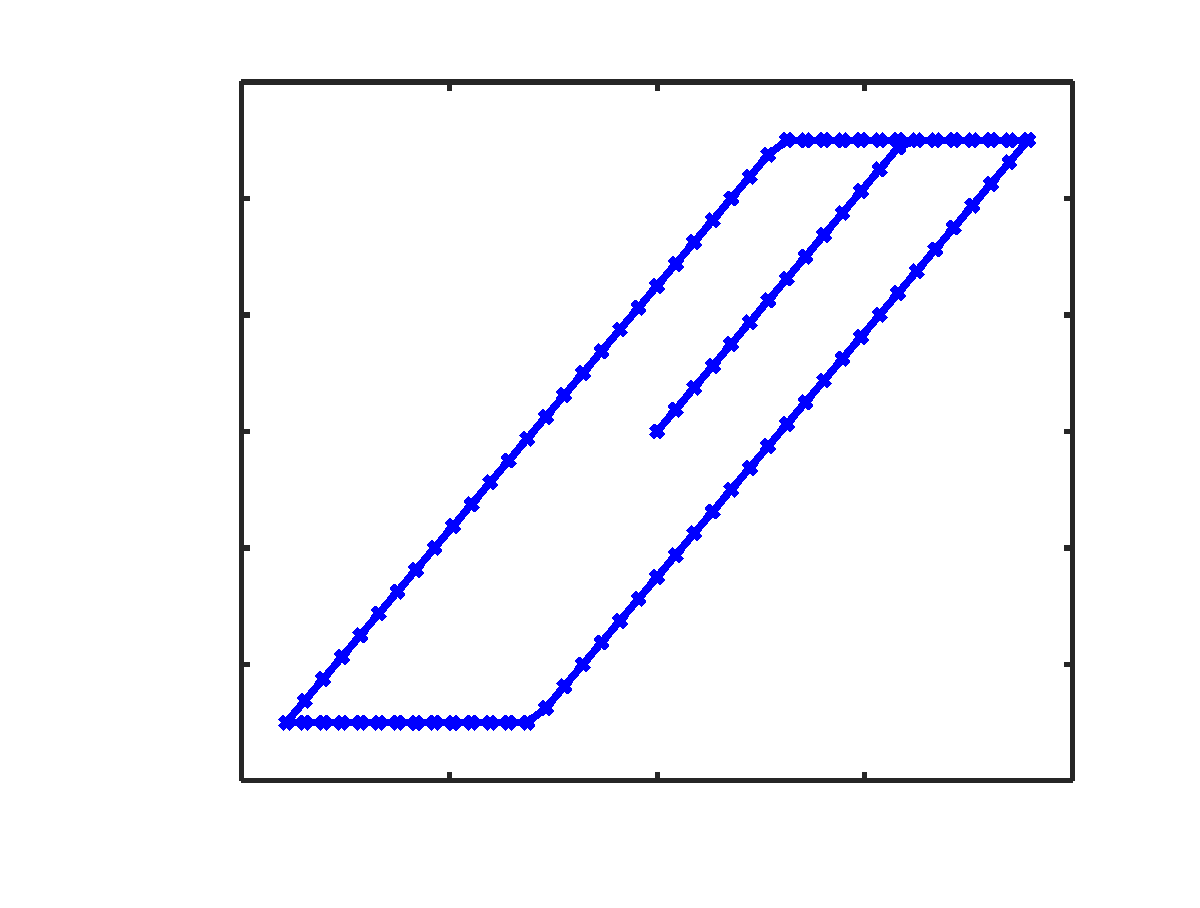
\includegraphics{plasticcycle-inc}
\end{picture}%
\begin{picture}(560,420)(0,0)
\fontsize{20}{0}
\selectfont\put(107.997,48.007){\makebox(0,0)[t]{\textcolor[rgb]{0.15,0.15,0.15}{{-0.002}}}}
\fontsize{20}{0}
\selectfont\put(207.698,48.007){\makebox(0,0)[t]{\textcolor[rgb]{0.15,0.15,0.15}{{-0.001}}}}
\fontsize{20}{0}
\selectfont\put(307.399,48.007){\makebox(0,0)[t]{\textcolor[rgb]{0.15,0.15,0.15}{{0}}}}
\fontsize{20}{0}
\selectfont\put(407.099,48.007){\makebox(0,0)[t]{\textcolor[rgb]{0.15,0.15,0.15}{{0.001}}}}
\fontsize{20}{0}
\selectfont\put(506.8,48.007){\makebox(0,0)[t]{\textcolor[rgb]{0.15,0.15,0.15}{{0.002}}}}
\fontsize{20}{0}
\selectfont\put(103,52.9996){\makebox(0,0)[r]{\textcolor[rgb]{0.15,0.15,0.15}{{-3e+08}}}}
\fontsize{20}{0}
\selectfont\put(103,108.916){\makebox(0,0)[r]{\textcolor[rgb]{0.15,0.15,0.15}{{-2e+08}}}}
\fontsize{20}{0}
\selectfont\put(103,164.833){\makebox(0,0)[r]{\textcolor[rgb]{0.15,0.15,0.15}{{-1e+08}}}}
\fontsize{20}{0}
\selectfont\put(103,220.75){\makebox(0,0)[r]{\textcolor[rgb]{0.15,0.15,0.15}{{0}}}}
\fontsize{20}{0}
\selectfont\put(103,276.667){\makebox(0,0)[r]{\textcolor[rgb]{0.15,0.15,0.15}{{1e+08}}}}
\fontsize{20}{0}
\selectfont\put(103,332.583){\makebox(0,0)[r]{\textcolor[rgb]{0.15,0.15,0.15}{{2e+08}}}}
\fontsize{20}{0}
\selectfont\put(103,388.5){\makebox(0,0)[r]{\textcolor[rgb]{0.15,0.15,0.15}{{3e+08}}}}
\fontsize{20}{0}
\selectfont\put(307.399,24.007){\makebox(0,0)[t]{\textcolor[rgb]{0.15,0.15,0.15}{{Deformacion}}}}
\fontsize{20}{0}
\selectfont\put(23.9999,220.75){\rotatebox{90}{\makebox(0,0)[b]{\textcolor[rgb]{0.15,0.15,0.15}{{Tension}}}}}
\end{picture}
}
	\resizebox{.48\linewidth}{!}{% Title: gl2ps_renderer figure
% Creator: GL2PS 1.4.0, (C) 1999-2017 C. Geuzaine
% For: Octave
% CreationDate: Wed Dec 27 09:12:51 2017
\setlength{\unitlength}{1pt}
\begin{picture}(0,0)
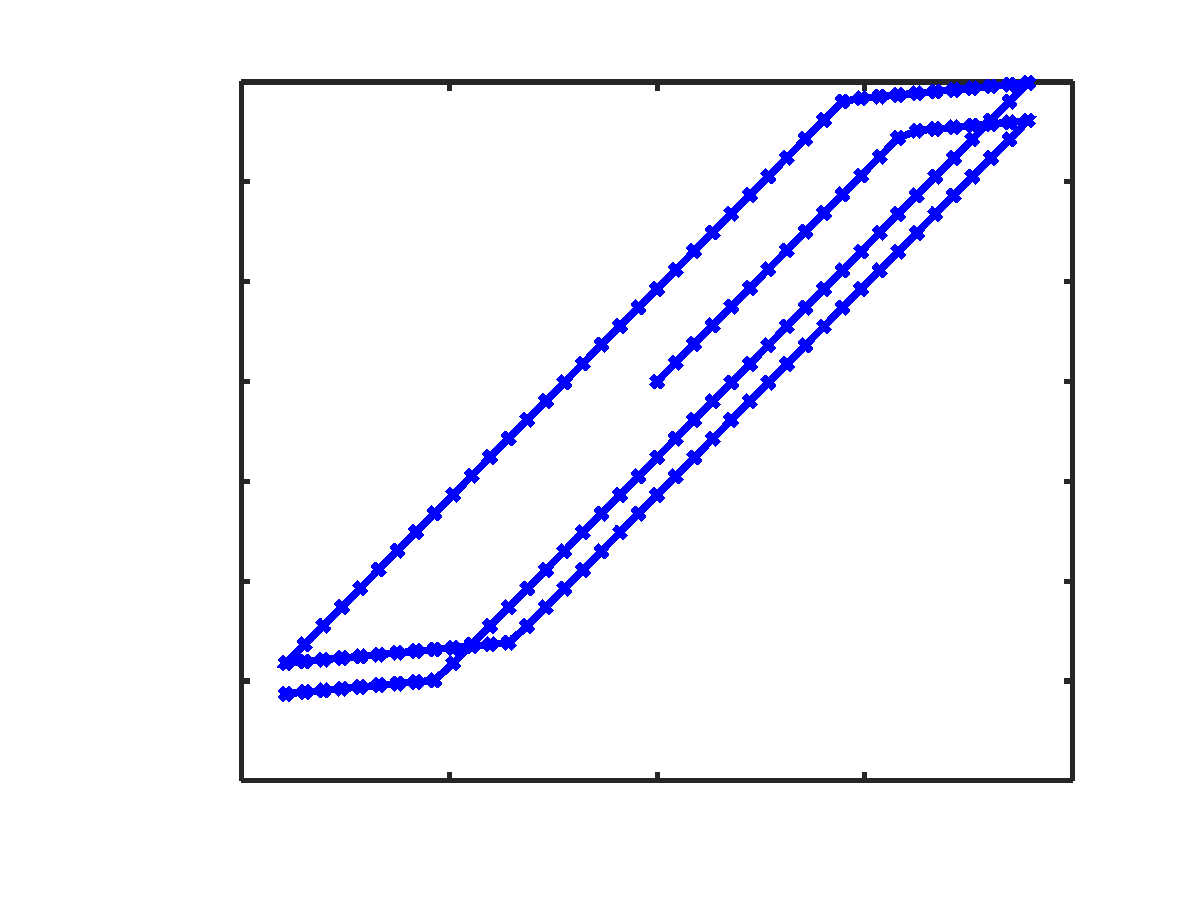
\includegraphics{plasticcycle2-inc}
\end{picture}%
\begin{picture}(560,420)(0,0)
\fontsize{20}{0}
\selectfont\put(107.997,48.007){\makebox(0,0)[t]{\textcolor[rgb]{0.15,0.15,0.15}{{-0.002}}}}
\fontsize{20}{0}
\selectfont\put(207.698,48.007){\makebox(0,0)[t]{\textcolor[rgb]{0.15,0.15,0.15}{{-0.001}}}}
\fontsize{20}{0}
\selectfont\put(307.399,48.007){\makebox(0,0)[t]{\textcolor[rgb]{0.15,0.15,0.15}{{0}}}}
\fontsize{20}{0}
\selectfont\put(407.099,48.007){\makebox(0,0)[t]{\textcolor[rgb]{0.15,0.15,0.15}{{0.001}}}}
\fontsize{20}{0}
\selectfont\put(506.8,48.007){\makebox(0,0)[t]{\textcolor[rgb]{0.15,0.15,0.15}{{0.002}}}}
\fontsize{20}{0}
\selectfont\put(103,52.9996){\makebox(0,0)[r]{\textcolor[rgb]{0.15,0.15,0.15}{{-4e+08}}}}
\fontsize{20}{0}
\selectfont\put(103,100.928){\makebox(0,0)[r]{\textcolor[rgb]{0.15,0.15,0.15}{{-3e+08}}}}
\fontsize{20}{0}
\selectfont\put(103,148.857){\makebox(0,0)[r]{\textcolor[rgb]{0.15,0.15,0.15}{{-2e+08}}}}
\fontsize{20}{0}
\selectfont\put(103,196.785){\makebox(0,0)[r]{\textcolor[rgb]{0.15,0.15,0.15}{{-1e+08}}}}
\fontsize{20}{0}
\selectfont\put(103,244.714){\makebox(0,0)[r]{\textcolor[rgb]{0.15,0.15,0.15}{{0}}}}
\fontsize{20}{0}
\selectfont\put(103,292.643){\makebox(0,0)[r]{\textcolor[rgb]{0.15,0.15,0.15}{{1e+08}}}}
\fontsize{20}{0}
\selectfont\put(103,340.571){\makebox(0,0)[r]{\textcolor[rgb]{0.15,0.15,0.15}{{2e+08}}}}
\fontsize{20}{0}
\selectfont\put(103,388.5){\makebox(0,0)[r]{\textcolor[rgb]{0.15,0.15,0.15}{{3e+08}}}}
\fontsize{20}{0}
\selectfont\put(307.399,24.007){\makebox(0,0)[t]{\textcolor[rgb]{0.15,0.15,0.15}{{Deformacion}}}}
\fontsize{20}{0}
\selectfont\put(23.9999,220.75){\rotatebox{90}{\makebox(0,0)[b]{\textcolor[rgb]{0.15,0.15,0.15}{{Tension}}}}}
\end{picture}
}
	\caption{Gráficos tensión-deformación de ejemplos de comportamiento elastoplástico: modelo elastoplástico perfecto (izq.) y modelo con endurecimiento lineal (der.).}
	\label{fig:grafsplast}
\end{figure}

Se observa, como era de esperar, que la tensión va aumentando conforme continúa el proceso de carga descarga. %
%
Esto es explicado por el hecho de que a pesar de que la deformación total se mantenga acotada, la deformación plástica acumulada durante el proceso continua aumentando. %
%
Si los resultados experimentales o el modelo constitutivo del material establecen algún valor de tensión de rotura, el mismo podría ser alcanzado luego de un cierto número de ciclos.

\subsection{Aplicación a reticulados}

El desarrollo presentado anteriormente puede ser aplicado al análisis de estructuras formadas por elementos con comportamiento elasto-plástico. %
%
Para esto, se debe incluir el cálculo de las magnitudes asociadas a la plastificación dentro de los algoritmos iterativos para encontrar la configuración de equilibrio. %
%
En el primer capítulo de \citep{Simo1998} se encuentra un desarrollo completo de los modelos unidimensionales y su integración en algoritmos basados en el MEF.

\section[Solicitaciones últimas en sección de hormigón armado] {Ejemplo: cálculo de solicitaciones últimas en sección de hormigón armado} 
%

En esta sección se presenta una breve discusión sobre análisis no lineal de secciones y se resuelve un ejemplo de cálculo de solicitaciones últimas en una sección de hormigón armado considerando el comportamiento no lineal del hormigón. %

A pesar de que el comportamiento del hormigón es usualmente considerado elastoplástico, en el ejemplo se considera un análisis elástico no lineal dado por una relación tensión-deformación sin calcular deformaciones plásticas. %
%
En el caso de que no se realice descarga este análisis elástico no lineal produce resultados iguales a los del análisis utilizando el modelo de elastoplasticidad. %
%
En el caso de que la estructura no se lleve a la falla, es decir que continúe en servicio luego de la descarga, este análisis no es útil, ya que se deben calcular o estimar las deformaciones remanentes correspondientes.

Es importante resaltar que este tipo de análisis no es un análisis no lineal completo de un elemento estructural. %
%
Para realizar un análisis no lineal de un elemento de viga se debe considerar la no linealidad no solamente en la sección transversal sino que también según el eje de la viga. %
%
En \citep{Liew2017,Lemes2017} se presentan resultados de análisis no lineales de elementos de viga de acero y hormigón considerando la relación momento-curvatura dada por el comportamiento constitutivo. %
%
Utilizando un procedimiento similar al presentado en este ejemplo es posible construir el diagrama momento-curvatura de una sección de hormigón considerando efectos de complejidad de modelado como por ejemplo fisuración. %
%
En \citep{Alhasawi2017} se realiza un análisis de pórticos considerando elementos de viga con rótulas elasto-plásticas en los extremos, aplicando conceptos de plasticidad como los vistos en la sección anterior.


En el ejemplo desarrollado a continuación se calculan los momentos y directas integrando el diagrama de tensiones de la sección utilizando integración numérica. %
%
Para la integración se utiliza el método de cuadratura de Gauss \citep{quarteroni2007numeric}, el cual permite calcular de forma eficiente las solicitaciones tal como se muestra en \citep{Bonet2006}.

Se considera una sección de hormigón armado de geometría rectangular de ancho $b=0.25$ m y altura $h= 0.6$ m con armadura simétrica dispuesta como se muestra en la Figura~\ref{fig:seccion}, con recubrimiento mecánico $r_m=0.06$ m. %
%
Los rectángulos oscuros representan barras de acero de refuerzo.
	
%
\begin{figure}[htb]
	\def\svgwidth{0.4\textwidth}
\input{../fig/seccion.pdf_tex}
	\caption{Esquema de sección transversal de hormigón armado.}
	\label{fig:seccion}
\end{figure}

El acero considerado es de tipo B500 y el hormigón es tipo C25 (resistencia característica $f_{ck}=25 $ N/mm$^2$). %

Se desea obtener las solicitaciones últimas resistidas por la sección para diferente cuantía, posición de linea neutra y curvatura, es decir los diagramas de interacción para la sección.

Para la resolución de este ejemplo nos guiaremos por el procedimiento descrito en \citep{JimenezMontoya}, material basado en la norma española EHE-2008\footnote{Enlace a norma en \href{http://www.fomento.es/MFOM/LANG_CASTELLANO/ORGANOS_COLEGIADOS/MASORGANOS/CPH/instrucciones/EHE_es/}{sitio web de ministerio de fomento español} (último acceso diciembre 2017).}. %
%
Para determinar las solicitaciones últimas soportadas por una sección rectangular se debe calcular las siguientes integrales
%
\begin{equation}
M_{\text{int}} = M_{\text{int}}^C + M_{\text{int}}^D = \int_{-\frac{h}{2}}^{\frac{h}{2}} b \, \sigma_x(y) \, y \, dy + \sum_{i=1}^{n_D} \sigma(y_i) \, y_i \, A_i 
\end{equation}
%
donde $M^C$ es el momento último dado por el hormigón (tensión continua en la altura) y $M^D$ es el momento producido por tensiones discretas (barras), $y_i$ y $A_i$ son las posiciones y áreas donde hay barras de acero, e $y$ vale cero en la mitad de la altura. %
%

Se considera además $y_1=-0.45h$, $y_2=0.45h$ y armadura simétrica ($A_1 = A_2 = A_s$). %

De forma análoga se calcula la directa resultante:
%
\begin{equation}  
N_{\text{int}} = N_{\text{int}}^C + N_{\text{int}}^D = \int_{-\frac{h}{2}}^{\frac{h}{2}} b \, \sigma_x(y) \,  dy + \sum_{i=1}^{n_{D}} \sigma(y_i) \, A_i 
\end{equation}
%

Pueden ser fácilmente implementadas funciones de Octave que permitan calcular los valores de directa y momento a partir de la curvatura y la posición de la linea neutra. %
%
A partir de dichas funciones, se pueden calcular las integrales numéricamente utilizando el método de cuadratura de Gauss, en este caso con cinco puntos de integración. %

Las integrales se calculan evaluando el integrando que depende de la función $\sigma(y)$. %
%
Esta función $\sigma(y)$ está dada a través de la ecuación constitutiva axial y la expresión de la deformación, es decir $\sigma (y) = \sigma( \varepsilon ( y) )$. %

La función de deformación en función de la distancia a la línea neutra  $y - y_{N}$ y la curvatura $\kappa$ se puede expresar de la siguiente forma:
%
\begin{equation}
\varepsilon(y) = - \kappa \, (y - y_{N} ) 
\end{equation}
%
donde $y_N$ es la posición de la linea neutra.

La ecuación constitutiva considerada para el hormigón es del tipo parábola-rectángulo, sin considerar resistencia a tracción, mientras que para el acero se utiliza un modelo elastoplástico perfecto. %
%
La expresión analítica de la ecuación constitutiva del hormigón es:
%
\begin{equation}
\sigma^C(\varepsilon) = %
\left\{ %
\begin{array}{lcl}
-f_{cd}  & \text{ si } & \varepsilon  \in [ -3.5 \text{\permil} , -2\text{\permil} ]  \\[2mm]
1000  \,.\, f_{cd}  \,.\, \varepsilon  \,.\, ( 250 \,.\, \varepsilon + 1)  & \text{si} & \varepsilon \in [  -2 \text{\permil} , 0] \\[2mm]
0  & \text{ si } & \varepsilon  > 0 \\[2mm]
\end{array}   \right.
\end{equation}
%
mientras que para el acero se tiene que la tensión de límite elástico es $\varepsilon_y = 2.17 \text{\permil}$ y por lo tanto la ecuación está dada por
%
\begin{equation}
\sigma^D(\varepsilon) = %
\left\{ %
\begin{array}{lcl}
E \, \varepsilon  & \text{si} & |\varepsilon| < 2,17 \text{\permil} \\[2mm]
f_{yd} \,. \, \text{signo}(\varepsilon) \quad & \text{si} & |\varepsilon| \geq 2,17 \text{\permil} \\[2mm]
\end{array}   \right.
\end{equation}
%
%Los códigos de las funciones de octave utilizados para evaluar estas funciones están presentados en la Sección~\ref{sec:cod2}. %

Las relaciones constitutivas del hormigón y el acero son representadas gráficamente en la Figura~\ref{fig:graficos_consitutivas} a la izquierda y derecha respectivamente.
%
\begin{figure}[htb]
	\centering
\def\svgwidth{0.95\textwidth}
\input{../fig/graficos_consitutivas.pdf_tex}
		\caption{Relaciones constitutivas de hormigón (izquierda) y acero (derecha).} \label{fig:graficos_consitutivas}
\end{figure}

Finalmente, se calculan las solicitaciones para los valores de linea neutra y curvatura dados por el diagrama de pivotes y con los valores obtenidos se construye el diagrama de interacción mostrado en la Figura~\ref{fig:interaccion}.

\setlength{\unitlength}{0.95\textwidth}
\begin{figure}[htb]
	\noindent
	\begin{center}
		\begin{picture}(1,0.75)%
		\put(0,0){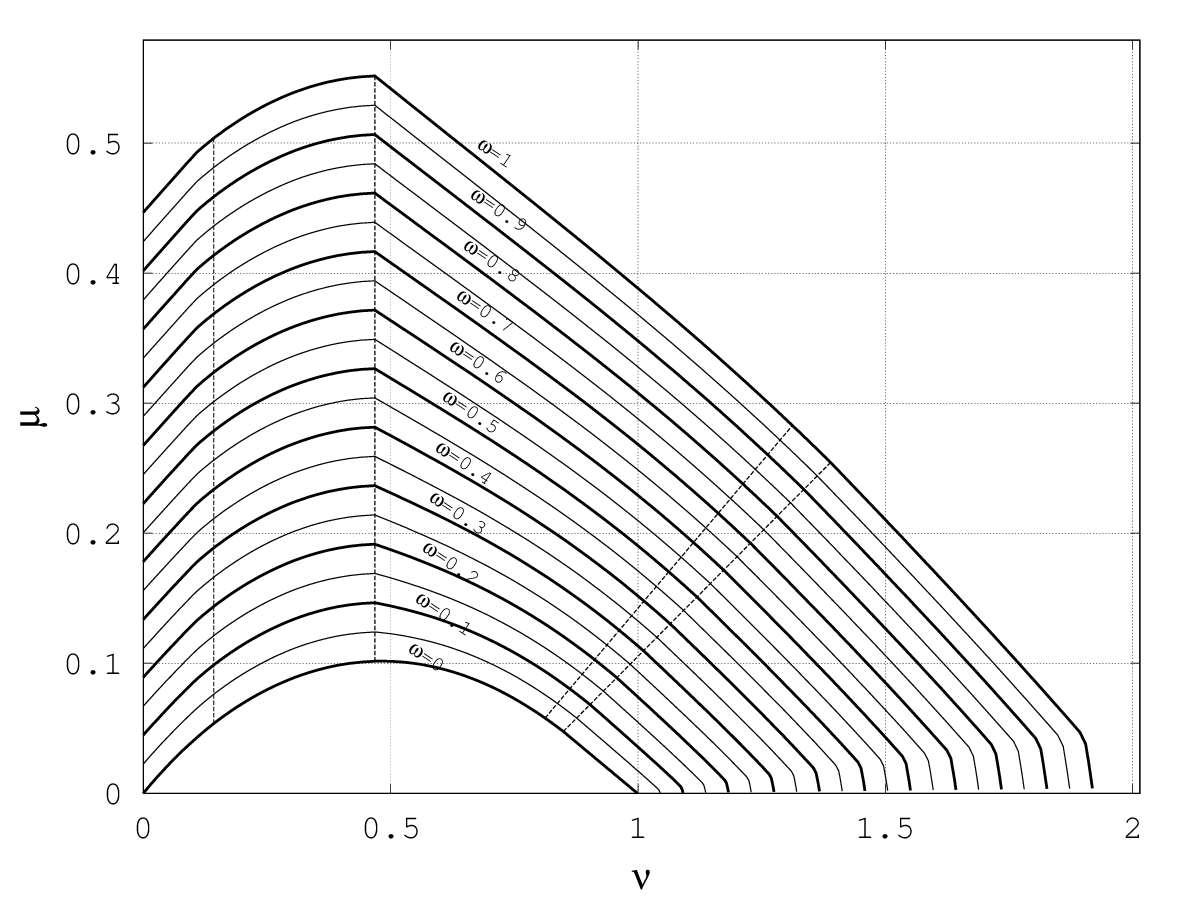
\includegraphics[width=\unitlength]{../fig/interaccion.pdf}}%
		\put(0.75,0.6){\color[rgb]{0,0,0}\makebox(0,0)[lb]{\smash{$\mu=\dfrac{M}{b h^2 f_{cd}}$}}}%
		\put(0.75,0.5){\color[rgb]{0,0,0}\makebox(0,0)[lb]{\smash{$\nu=\dfrac{N}{b h f_{cd}}$}}}%
		\put(0.75,0.4){\color[rgb]{0,0,0}\makebox(0,0)[lb]{\smash{$\omega = \dfrac{A f_{yd} }{b h f_{cd}}$}}}%
		\end{picture}%
		\caption{Diagrama de interacción de sección rectangular de hormigón armado.} \label{fig:interaccion}
	\end{center}
\end{figure}

Los ejes del gráfico muestran los momentos y directas reducidos, $\mu$ y $\nu$ respectivamente y las líneas punteadas conectan los puntos $(\nu,\mu)$ en los cuales se produce el cambio de dominio en el diagrama de pivotes para las distintas cuantías consideradas.

\cajaactividad{Comparar el diagrama de interacción obtenido con el correspondiente presentado en \citep{JimenezMontoya}.}

